%%
% Please see https://bitbucket.org/rivanvx/beamer/wiki/Home for obtaining beamer.
%%
%\documentclass[11pt,aspectratio=169]{beamer}
%\documentclass[11pt,aspectratio=169,xcolor={dvipsnames}]{beamer}

\documentclass[11pt,aspectratio=169,xcolor={dvipsnames},hyperref={pdftex,pdfpagemode=UseNone,hidelinks,pdfdisplaydoctitle=true},usepdftitle=false]{beamer}
\usepackage{presentation}


\title{Lecture 13: Costly State Verification}
\author{Juan Herre\~{n}o\\UCSD}
\date{2026}

% Enter presentation title to populate PDF metadata:
\newcommand{\Cov}{\text{Cov}_\lambda}
\newcommand{\El}{\mathbb{E}_\lambda}
\newcommand{\mm}{\text{{\fontfamily{qzc}\selectfont m}}}
\usepackage{cancel}
\usepackage{booktabs}
\begin{document}

\maketitle


\begin{frame}{Financial Markets}
\begin{itemize}
	\itemsep1em 
	\item Core role of financial markets:
	\begin{itemize}
		\item Match savers with borrowers
		\item Allow funds to flow from those that have more funds than projects \\ to those that have more projects than funds
	\end{itemize}
	\item Core friction in financial markets:
	\begin{itemize}
		\item Agency problem with asymmetric information
		\item Savers know less about projects than borrowers
		\item Borrowers can take too much risk / put in too little effort / lie about outcome (moral hazard)
\item Savers cannot observe the borrower or project ``type'' (adverse selection)
	\end{itemize}
\end{itemize}
\end{frame}


\begin{frame}{Costly State Verification Model}
\begin{itemize}
	\itemsep1em 
\item The entrepreneur has a project that requires 1 unit of resources
\item The entrepreneur has wealth $W<1$
\item They must obtain $1-W$ of outside financing
\item The expected output of the project is $\gamma$
	\begin{itemize}
		\item Heterogeneous across projects
		\item Publicly observable (no adverse selection) 
	\end{itemize}
	\item Actual output is distributed $Y \sim U [0, 2\gamma]$	
\end{itemize}
\end{frame}


\begin{frame}{Costly State Verification Model}
\begin{itemize}
	\itemsep1em 
	\item Outside investor must bear some risk
	\begin{itemize}
		\item Output realization can be lower than $1-W$
	\end{itemize}
	\item For simplicity: Entrepreneur and investor are risk neutral
	\item Outside option: Technology that yields a net return of $r$
	\item Perfect competition among outside investors
	\begin{itemize}
		\item Implies expected net return to outside investors is $r$
	\end{itemize}
\end{itemize}
\end{frame}


\begin{frame}{Costly State Verification Model}
\begin{itemize}
	\itemsep1em 
	\item Socially efficient to undertake project if $\gamma > 1+r$
	\item Entrepreneur undertakes project if
	\[ E[Y - P] > (1+r) W \]
	where $P$ denotes payments to outside investor
\end{itemize}
\end{frame}


\begin{frame}{Costly State Verification Model}
\begin{itemize}
	\itemsep1em 
	\item Entrepreneur knows actual output but investor does not
	\item Outside investor must pay $c$ to verify actual output
	\item Costly state verification model of asymmetric information \\ {\small (Townsend, 1979)}
\end{itemize}
\end{frame}


\begin{frame}{Equilibrium with Symmetric Information}
\begin{itemize}
	\itemsep1em 
	\item Claim: Projects with $\gamma \geq 1+r$ get financing, others do not.
	\item Outside investor gets an expected payment $(1+r)(1-W)$ \pause 
	\item Many contracts can achieve this: Equity contract is one! \pause
	\begin{itemize}
		\item Outside investor gets fraction $(1+r)(1-W)/\gamma$ of output
		\[ E\left[\frac{(1+r)(1-W)}{\gamma}Y \right] = (1+r)(1-W) \]
	\end{itemize} \pause 
	\item Entrepreneur's expected income is 
	\[\gamma - (1+r)(1-W) = (1+r)W + \gamma - (1+r) \]
	which exceeds $(1+r)W$ if $\gamma \geq 1+r$, so entrepreneur is better off
\end{itemize}
\end{frame}


\begin{frame}{Optimal Contract with Asymmetric Info}
\begin{itemize}
	\itemsep1em 
\item With asymmetric information, the outside investor may need to verify output
	\item Expected payments to outside investor:
	\[ (1+r)(1-W) + \text{expected cost of verifying output} \]
	\item Efficiency dictates minimizing the cost of verifying output
	\item Entrepreneur gets output (exogenous) minus payments to investor
	\begin{itemize}
		\item Wants to minimize payments to outside investor
		\item Which means minimizing fraction of time investor \\ needs to verifying output
	\end{itemize}
\end{itemize}
\end{frame}


\begin{frame}{Optimal Contract with Asymmetric Info}
\begin{itemize}
	\itemsep1em 
	\item Optimal contract: Simple debt contract
	\begin{itemize}
		\item If $Y \geq D$, investor gets $D$ and does not verify output
		\item If $Y < D$, investor verifies output and gets $Y$
	\end{itemize}
	\item Intuitively:
	\begin{itemize}
		\item Entrepreneur ``borrows'' $1-W$
		\item Pays back $D$ when she can
		\item Defaults when $Y < D$ \\ (in which case investor verifies output and gets all of it)
	\end{itemize}
\end{itemize}
\end{frame}


\begin{frame}
\begin{figure}
	\centering
	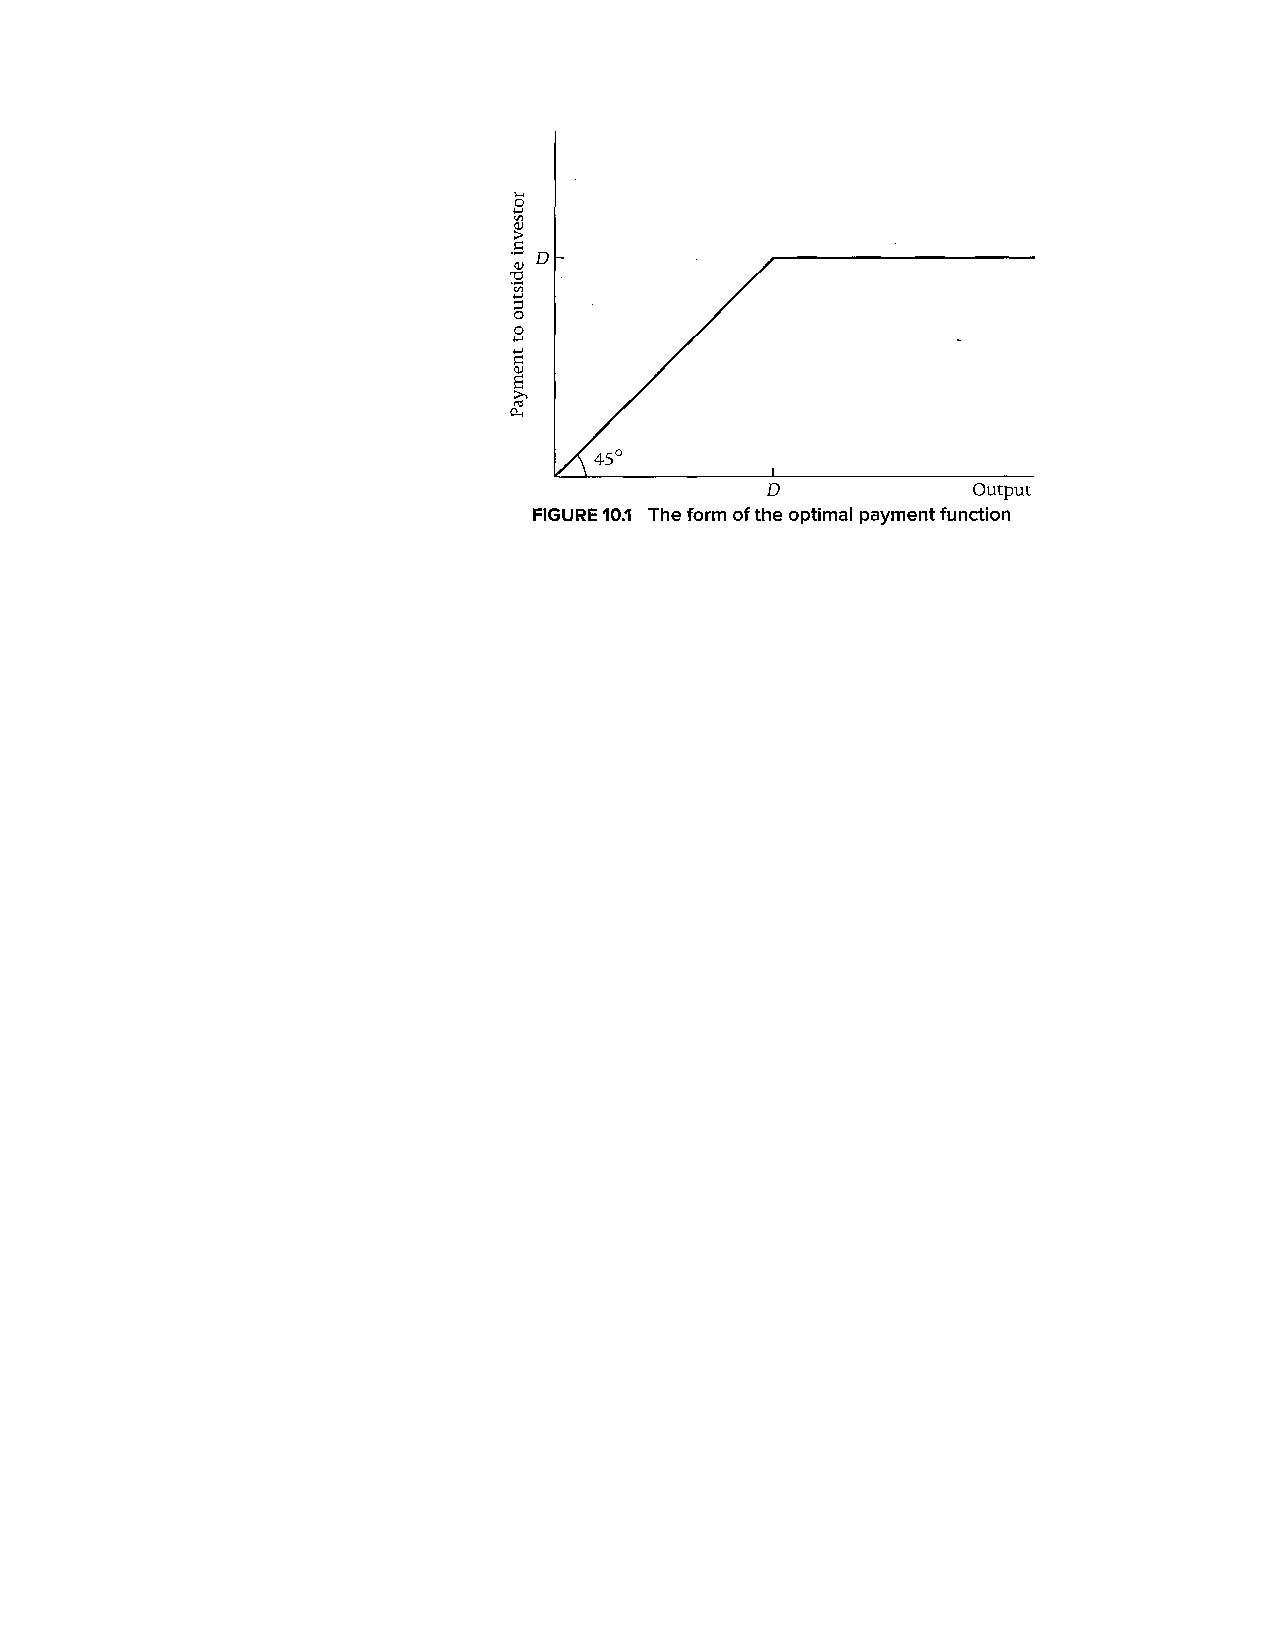
\includegraphics[height=0.9 \textheight]{FiguresTables/Romer2019Figure101.pdf}
\end{figure}
\vspace{-4mm}
{\scriptsize Source: Romer (2019)}
\end{frame}


\begin{frame}{Why Debt?}
\begin{itemize}
	\itemsep1em 
	\item When investor does not verify output, payment cannot \\ depend on actual output
	\begin{itemize}
		\item Entrepreneur would have an incentive to misreport
		\item Always report lowest non-verified output level
	\end{itemize}
	\item Payment with verification cannot exceed payment without verification
	\begin{itemize}
		\item Entrepreneur would have an incentive to misreport
		\item Always report non-verified output levels when output is at higher levels
	\end{itemize}
	\item Payment with verification cannot equal $D$
	\begin{itemize}
		\item Might as well not verify and save verification cost
	\end{itemize}
\end{itemize}
\end{frame}


\begin{frame}{Why Debt?}
\vspace{10pt}
\begin{itemize} \addtocounter{enumi}{3}
	\itemsep1em 
	\item Payment is $D$ whenever output exceeds $D$
	\begin{itemize}
		\item If lower, possible to increase investor's expected returns and \\ lower expected verification costs by raising payment to $D$
	\end{itemize}
	\item Investor must verify if output is less than $D$
	\begin{itemize}
		\item Entrepreneur cannot pay $D$ in this case
		\item So, investor must verify
	\end{itemize}
	\item Payment equals output if output is less than $D$
	\begin{itemize}
		\item If lower, possible to increase investor's expected returns and \\ lower expected verification costs by raising payment to $Y$
	\end{itemize}
\end{itemize}
\vspace{10pt}
{\footnotesize Optimal \textit{pure strategy} contract. Subgame perfect? Bankcruptcy as commitment device?}
\end{frame}


\begin{frame}{Investor Expected Net Revenue}
\[ R(D) = \left\{ \begin{array}{lll} 
\frac{2\gamma - D}{2\gamma} D + \frac{D}{2\gamma} \left( \frac{D}{2} - c \right) & \text{if} & D \leq 2\gamma \\
\gamma - c & \text{if} & D > 2\gamma
\end{array} \right. \] 
\begin{itemize}
	\item Recall that $Y \sim U[0,2\gamma]$
	\item If $D\leq 2\gamma$ probability output is above $D$ is $(2\gamma-D)/(2\gamma)$
	\item Expected output if $Y<D$ is $D/2$ 
\end{itemize}
\end{frame}


\begin{frame}
\begin{figure}
	\centering
	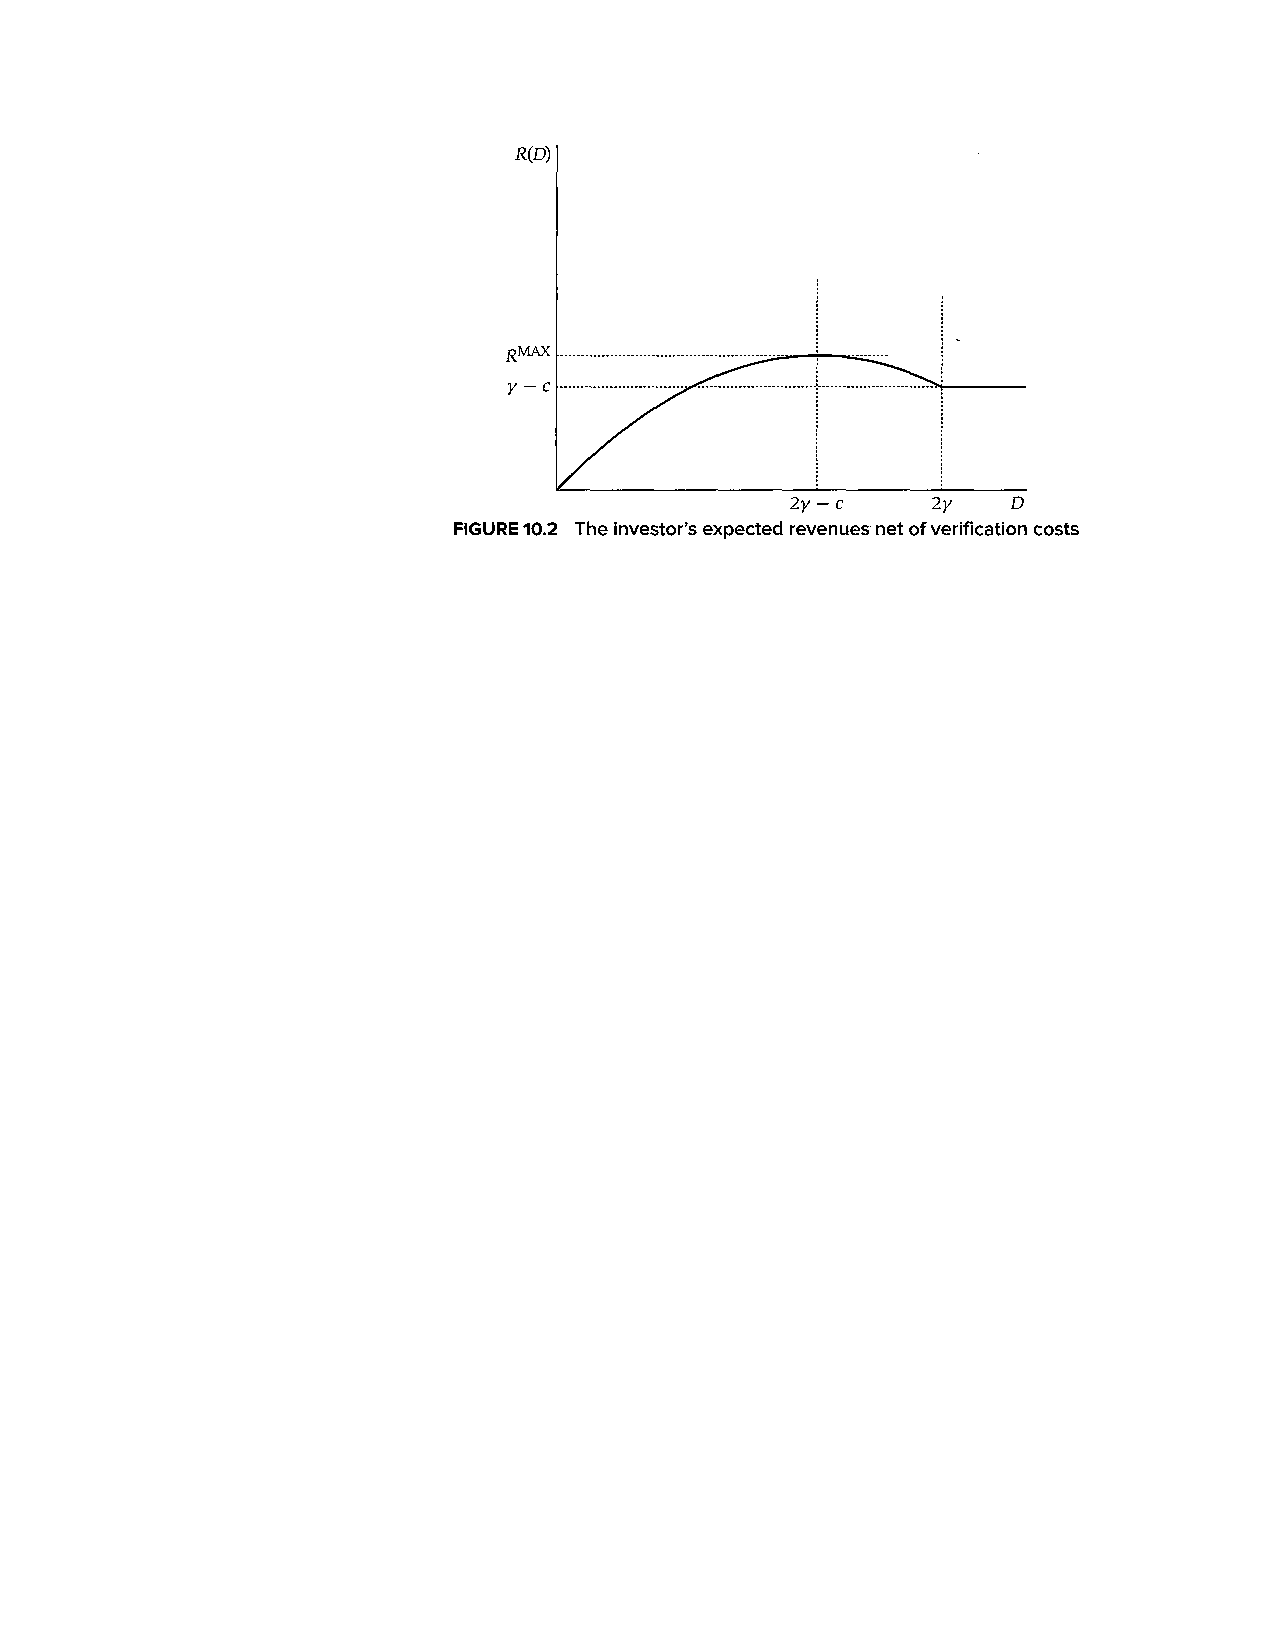
\includegraphics[height=0.8 \textheight]{FiguresTables/Romer2019Figure102.pdf}
\end{figure}
\vspace{-4mm}
{\scriptsize Source: Romer (2019). Raising $D$ above $2\gamma - c$ is not worth the extra verification cost.}
\end{frame}

\begin{frame}
\begin{figure}
	\centering
	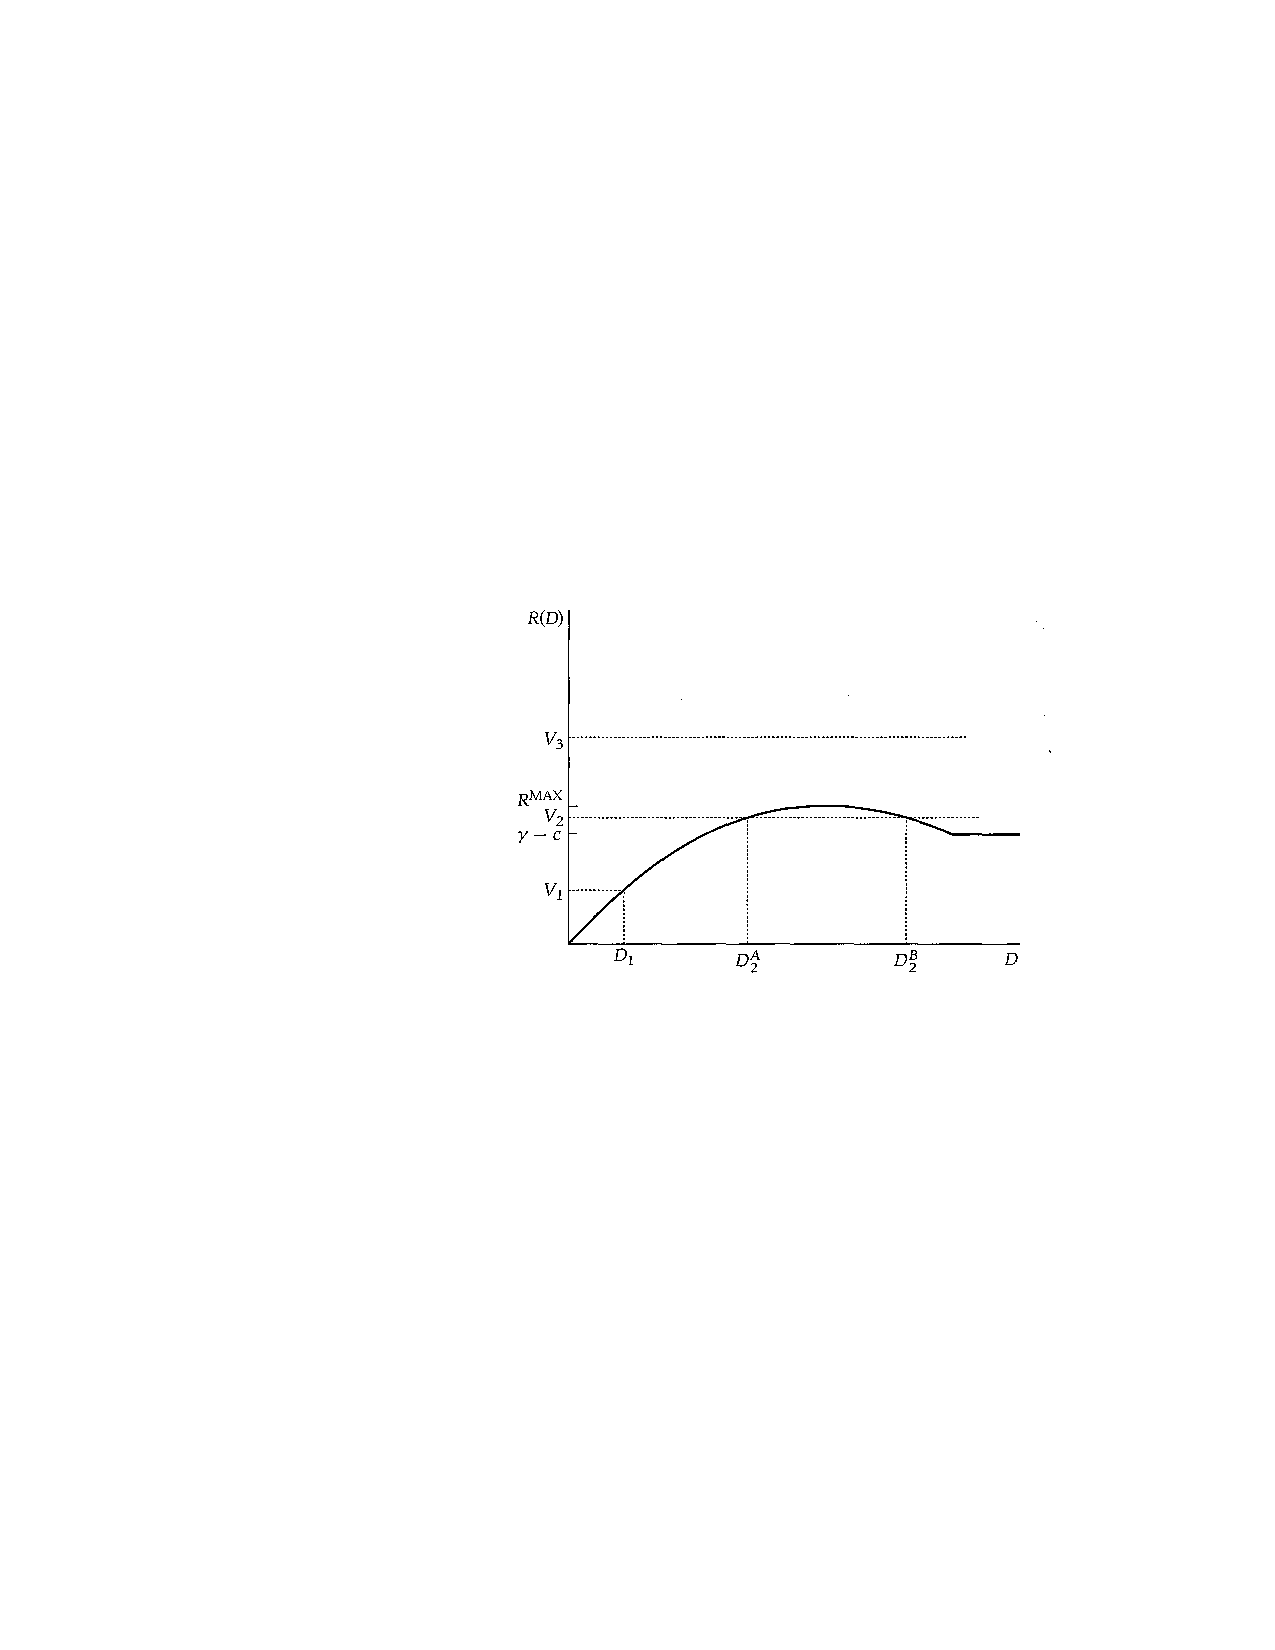
\includegraphics[height=0.8 \textheight]{FiguresTables/Romer2019Figure103.pdf}
\end{figure}
\vspace{-4mm}
{\scriptsize Source: Romer (2019). $V_1$, $V_2$, $V_3$ are three levels of required revenue $(1+r)(1-W)$.}
\end{frame}


\begin{frame}{Determination of $D$}
\begin{itemize}
	\itemsep1em 
	\item If required net revenue $(1+r)(1-W)$ exceed $R^{MAX}$, project not funded
	\begin{itemize}
		\item Required net revenue is decreasing in entrepreneur's wealth $W$
		\item Example of \textbf{credit rationing} as a function of $W$
	\end{itemize}
	\item If required net revenue below $R^{MAX}$, project funded and \\ equilibrium value of $D$ given by smaller solution to 
	\[ R(D) = (1+r)(1-W) \] 
	which is
	\[D^{*} = 2\gamma - c - \sqrt{(2\gamma - c)^{2} - 4\gamma(1+r)(1-W)} \] 
	{\footnotesize (Competition among investors drives D down to lower value)}
\end{itemize}
\end{frame}


\begin{frame}{Expected Verification Costs}
\begin{itemize}
	\item Expected verification costs are 
	\[\begin{array}{rcl} 
	A(c,r,W,\gamma) & = & \frac{D^{*}}{2\gamma} c \\
	  & = & \left[ \frac{2\gamma - c}{2\gamma} - \sqrt{\left(\frac{2\gamma - c}{2\gamma} \right)^{2} - \frac{(1+r)(1-W)}{\gamma} } \right] c
	\end{array} \]
	\item Derivatives of $A(c,r,W,\gamma)$:
	\[A_c > 0, \;\;\; A_r > 0, \;\;\; A_W < 0, \;\;\; A_{\gamma} < 0 \] 
\end{itemize}
\end{frame}


\begin{frame}{Will Project Be Undertaken?}
Project will be undertaken if:
\begin{itemize}
	\item Investor willing to lend:
	\[ R^{MAX} \geq (1+r)(1-W) \]
	\item Entrepreneur's return above outside option:
	\[ \gamma - (1+r)(1-W) - A(c,r,W,\gamma) \geq  (1+r)W \] 
\end{itemize}
\end{frame}


\begin{frame}{Will Project Be Undertaken?}
\begin{itemize}
	\itemsep1em
	\item With symmetric information project undertaken if $\gamma \geq (1+r)$
	\item With asymmetric information, other considerations come into play
	\item Entrepreneur's wealth matters
	\begin{itemize}
		\item Easier to finance when entrepreneur has more wealth \\ (more skin in the game)
		\item Less debt means lower $D^{*}$ and therefore less default/verification
	\end{itemize}
\end{itemize}
\end{frame}


\begin{frame}{Cost of Outside Finance}
\begin{itemize}
	\item Cost of outside finance higher than of inside finance
	\begin{itemize}
		\item Cost of inside finance:
		\[ 1+r \] 
		\item Cost of outside finance
		\[ 1+r + \frac{A(c,r,W,\gamma)}{1-W} \] 
	\end{itemize}
\end{itemize}
\end{frame}


\begin{frame}
\begin{figure}
	\centering
	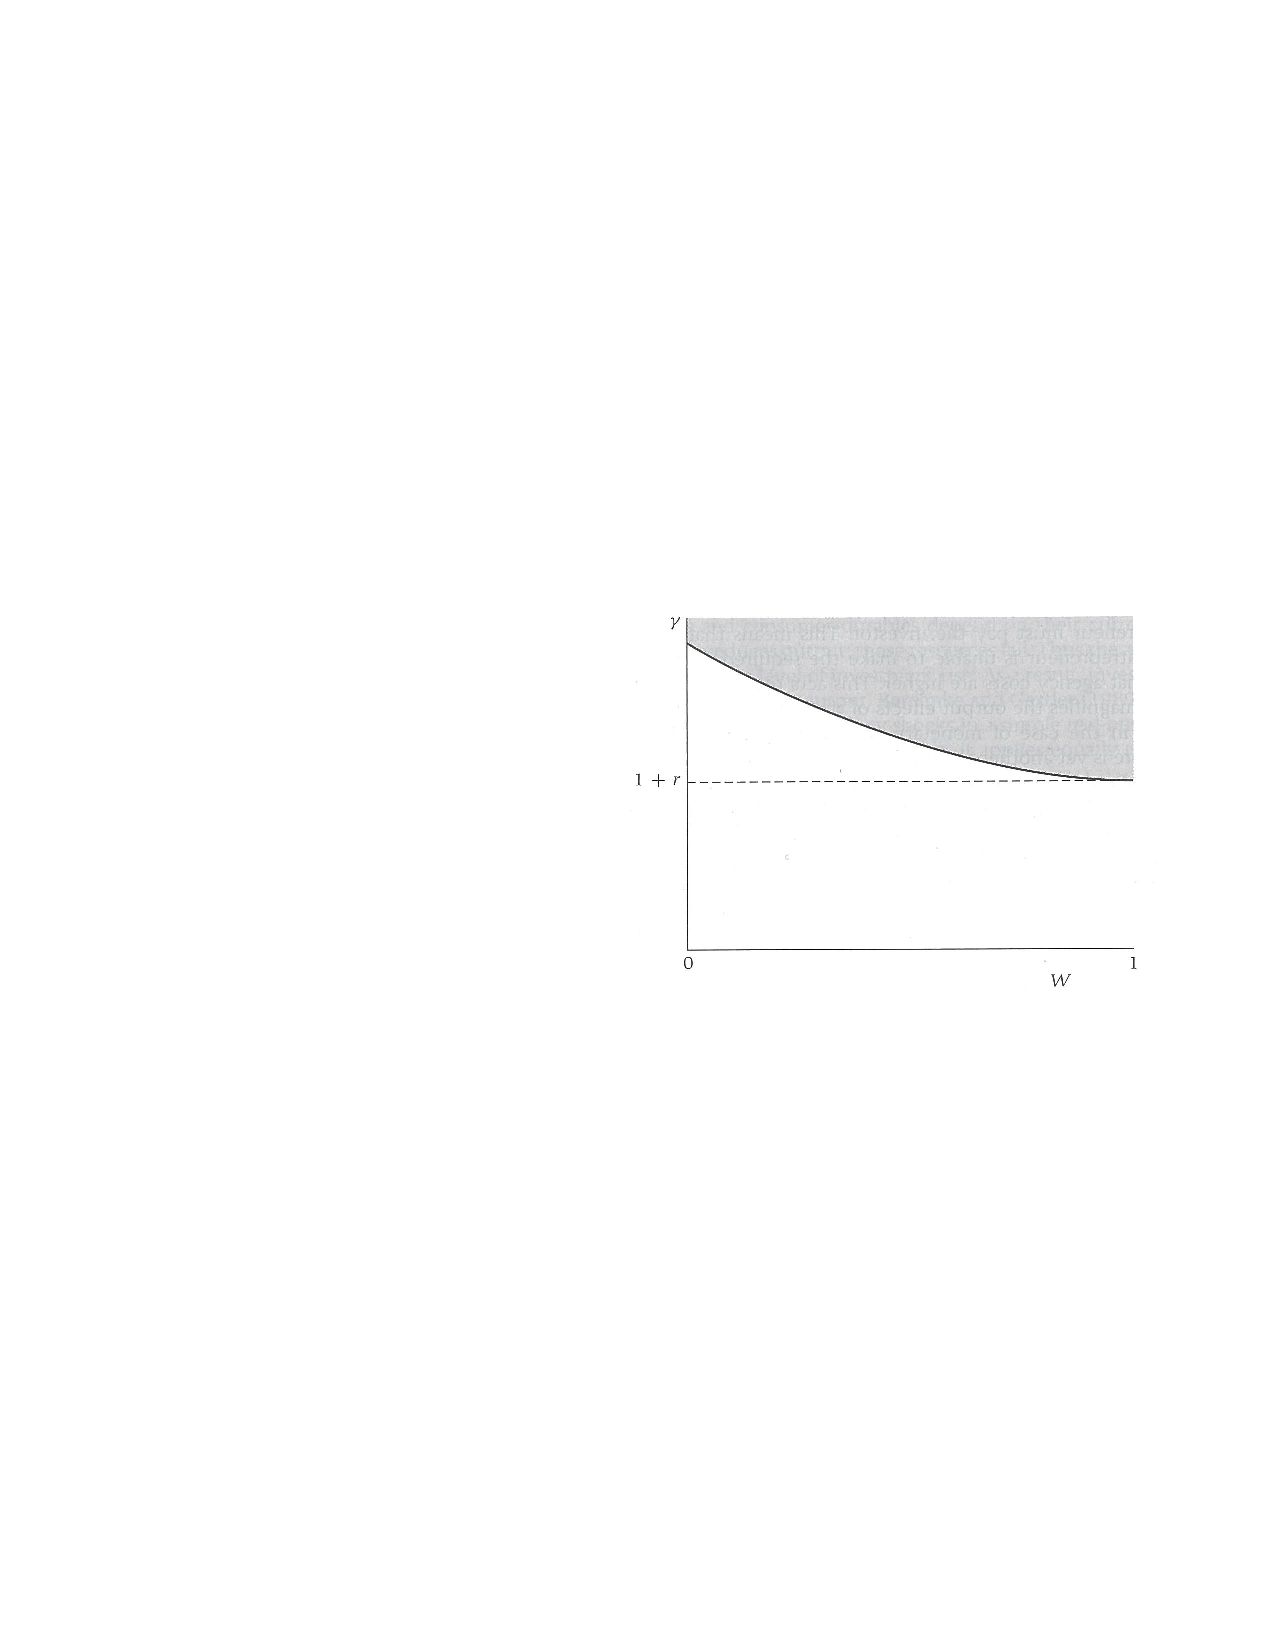
\includegraphics[height=0.85 \textheight]{FiguresTables/Romer2019Figure104.pdf}
\end{figure}
\vspace{-4mm}
{\scriptsize Source: Romer (2019).}
\end{frame}


\begin{frame}{Will Project Be Undertaken?}
\begin{itemize}
	\itemsep1em 
	\item Financial system itself matters for whether projects are funded
	\item An increase in verification cost $c$ reduces investment
	\item Two interpretations:
	\begin{itemize}
		\itemsep0.5em
		\item Efficiency of financial system in processing information and \\ monitoring borrowers is important for investment
		\item Financial system itself needs funding
		\begin{itemize}
			\item Shocks to the financial system increase its cost of outside finance \\ and reduce its ability to fund investment (e.g., Gertler-Kiyotaki 11)
			\item Large empirical literature (e.g., Peek-Rosengren 00,  Khwaja-Mian 08, Chodorow-Reich 14, Huber 18)
		\end{itemize}
	\end{itemize}
\end{itemize}
\end{frame}


\begin{frame}{Financial Accelerator}
\begin{itemize}
	\itemsep1em 
	\item Financial frictions amplify macro shocks
	\begin{itemize}
		\item Bad shock lowers profitability and entrepreneurial wealth
		\item Increases agency costs
		\item Resulting fall in investment amplifies initial shock
	\end{itemize}
	\item Feedback loop can cause large amplification
	\begin{itemize}
		\item Fall in investment can further weaken profitability and \\ entrepreneurial wealth (especially in a Keynesian model)
		\item Further increases agency costs and weakens investment.  
	\end{itemize}
	\item Strong enough feedback can result in multiple equilibria
	\item Key theoretical references: {\small Bernanke-Gertler 89, Kiyotaki-Moore 97, Bernanke-Gertler-Gilchrist 99}
\end{itemize}
\end{frame}

\end{document}




